\documentclass{article}
\usepackage{graphicx}
\usepackage{caption}
\usepackage{subcaption}
\usepackage{hyperref}
\graphicspath{{./figs/}}{}
\usepackage{listings}
\title{
HLS-Assignment 9 PART-2
}
\begin{document}

\maketitle
\hfill \textbf{VIVADO-VERILOG}
\section{Problem Statement}
\href{run:./problem_statement.pdf} {Problem Statemt}
\vspace{1cm}

\section{CRC bits Generator Code}
\begin{lstlisting}
//crcaxis.v
`timescale 1ns / 1ps

module axis_reg #(
        parameter integer DW_IN = 8,
        parameter integer DW_OUT = 32
    )
    (
        
        input wire clk,
        input wire reset_n,
        input wire [DW_IN - 1:0] s_tdata,
        input wire s_tvalid,
        output wire s_tready,
        output wire [DW_IN - 1:0] m_tdata,
        output wire m_tvalid,
        input wire m_tready
    );
    
    reg m_tvalid_i;
    reg [0:24] divisor = 25'b1100001100100110011111011;
    reg [0:31] crc_reg,crc_own;
    reg [1:0] cycle_counter;
    reg [7:0] oup;
    integer i, j;

    always @(posedge clk) begin
        if(!reset_n) begin
            m_tvalid_i <= 0;
            crc_reg <= 0;
            crc_own<=0;
            cycle_counter<=0;
        end else if(s_tready && s_tdata!=8'b00000001) begin
             crc_reg  = {s_tdata,{24{1'b0}}};
    
    for (i = 0; i <=7; i = i + 1) begin
      if (crc_reg[i] == 1) begin
        for (j = 0; j < 25; j = j + 1) begin
          crc_reg[i + j] = crc_reg[i + j] ^ divisor[j];
        end
      end
    end
    end
    crc_own = {s_tdata,crc_reg[8:31]};
    oup=crc_own[7+(8*cycle_counter) -:8];
    cycle_counter = cycle_counter + 1;
        
    end

    assign m_tdata = oup;
    assign m_tvalid = m_tdata?1:0;
    assign s_tready = m_tready || !m_tvalid;
endmodule

endmodule
\end{lstlisting}
\vspace{13cm}

\section{Test Bench Code}
\begin{lstlisting}
//axistb.v
`timescale 1ns / 1ps
//////////////////////////////////////////////////////////////////////////////////
// Company: 
// Engineer: 
// 
// Create Date: 06/27/2023 10:47:14 AM
// Design Name: 
// Module Name: axistb
// Project Name: 
// Target Devices: 
// Tool Versions: 
// Description: 
// 
// Dependencies: 
// 
// Revision:
// Revision 0.01 - File Created
// Additional Comments:
// 
//////////////////////////////////////////////////////////////////////////////////


module axistb(

    );
    reg clk;
    reg reset_n;
    reg [7:0] s_tdata;
    reg s_tvalid;
    wire s_tready;
    wire [7:0] m_tdata;
    wire m_tvalid;
    reg m_tready;
    
    // Instantiating
   axis_reg #(
        .DW_IN(8),
        .DW_OUT(32)
    ) dut (
        .clk(clk),
        .reset_n(reset_n),
        .s_tdata(s_tdata),
        .s_tvalid(s_tvalid),
        .s_tready(s_tready),
        .m_tdata(m_tdata),
        .m_tvalid(m_tvalid),
        .m_tready(m_tready)
    );
  /*   design_1_wrapper uut
   (.clk_0(clk),
    .m_0_tdata(m_tdata),
    .m_0_tvalid(m_tvalid),
    .reset_n_0(reset_n),
    .s_0_tdata(s_tdata),
    .s_0_tready(s_tready),
    .s_0_tvalid(s_tvalid),
    .m_0_tready(m_tready));
    */
    // Clock generation
    always #5 clk = ~clk;
    
    initial begin
        // Initialize inputs
        clk = 0;
        reset_n = 1;
        s_tdata = 8'h00;
        s_tvalid = 0;
        
        
        // Apply reset
        reset_n <= 0;
        #10;
        reset_n <= 1;
        m_tready<=1;
        
        
        // Send data and wait for it to be accepted
        s_tdata <= 8'b01101000;
        #10
        s_tdata <= 8'b00000001;
        #10 
        s_tdata <=8'dx;
        
        s_tvalid <= 1;
        #10;
        s_tvalid <= 0;
        #20
        m_tready<=0;
        #5
        // Finish simulation
        $finish;
    end

endmodule


\end{lstlisting}
\vspace{1cm}

\section{Output Waveform}
\vspace{1cm}
\begin{figure}[h]
    \centering
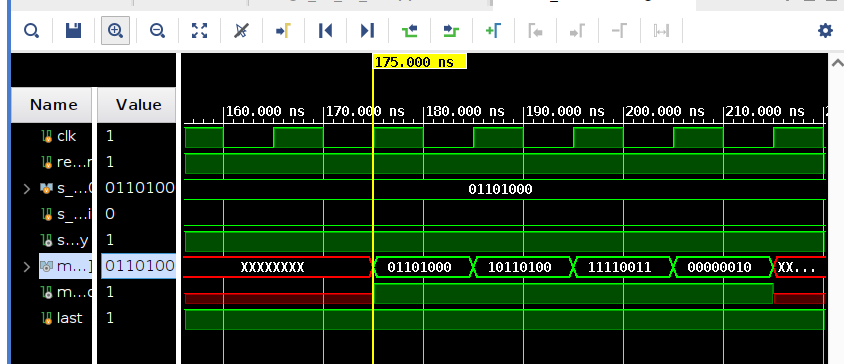
\includegraphics[width=\columnwidth]{figs/p2rtlwav.png}
    \caption{Output of RTL Testbench}
    \label{fig:my_label}
\end{figure}

\vspace{20cm}


\maketitle
\hfill \textbf{VIVADO-IP}
\section{Block Design}
\vspace{1cm}
\begin{figure}[h]
    \centering
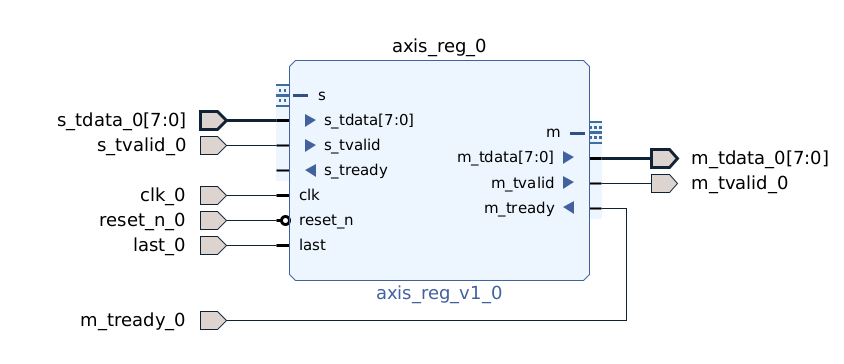
\includegraphics[width=\columnwidth]{figs/p2ipbd.png}
    \caption{Block Diagram}
    \label{fig:my_label}
\end{figure}
\vspace{3cm}
\section{Verilog Testbench}
\begin{lstlisting}
//axistb.v
`timescale 1ns / 1ps
//////////////////////////////////////////////////////////////////////////////////
// Company: 
// Engineer: 
// 
// Create Date: 06/27/2023 10:47:14 AM
// Design Name: 
// Module Name: axistb
// Project Name: 
// Target Devices: 
// Tool Versions: 
// Description: 
// 
// Dependencies: 
// 
// Revision:
// Revision 0.01 - File Created
// Additional Comments:
// 
//////////////////////////////////////////////////////////////////////////////////


module axistb(

    );
    reg clk;
    reg reset_n;
    reg [7:0] s_tdata;
    reg s_tvalid;
    wire s_tready;
    wire [7:0] m_tdata;
    wire m_tvalid;
    reg m_tready;
    
    // Instantiating
 /*  axis_reg #(
        .DW_IN(8),
        .DW_OUT(32)
    ) dut (
        .clk(clk),
        .reset_n(reset_n),
        .s_tdata(s_tdata),
        .s_tvalid(s_tvalid),
        .s_tready(s_tready),
        .m_tdata(m_tdata),
        .m_tvalid(m_tvalid),
        .m_tready(m_tready)
    );*/
     design_1_wrapper uut
   (.clk_0(clk),
    .m_0_tdata(m_tdata),
    .m_0_tvalid(m_tvalid),
    .reset_n_0(reset_n),
    .s_0_tdata(s_tdata),
    .s_0_tready(s_tready),
    .s_0_tvalid(s_tvalid),
    .m_0_tready(m_tready));
    
    // Clock generation
    always #5 clk = ~clk;
    
    initial begin
        // Initialize inputs
        clk = 0;
        reset_n = 1;
        s_tdata = 8'h00;
        s_tvalid = 0;
        
        
        // Apply reset
        reset_n <= 0;
        #10;
        reset_n <= 1;
        m_tready<=1;
        
        
        // Send data and wait for it to be accepted
        s_tdata <= 8'b01101000;
        #10
        s_tdata <= 8'b00000001;
        #10 
        s_tdata <=8'dx;
        
        s_tvalid <= 1;
        #10;
        s_tvalid <= 0;
        #20
        m_tready<=0;
        #5
        // Finish simulation
        $finish;
    end

endmodule

\end{lstlisting}

\vspace{1cm}


\section{Output Waveform}
\vspace{1cm}
\begin{figure}[h]
    \centering
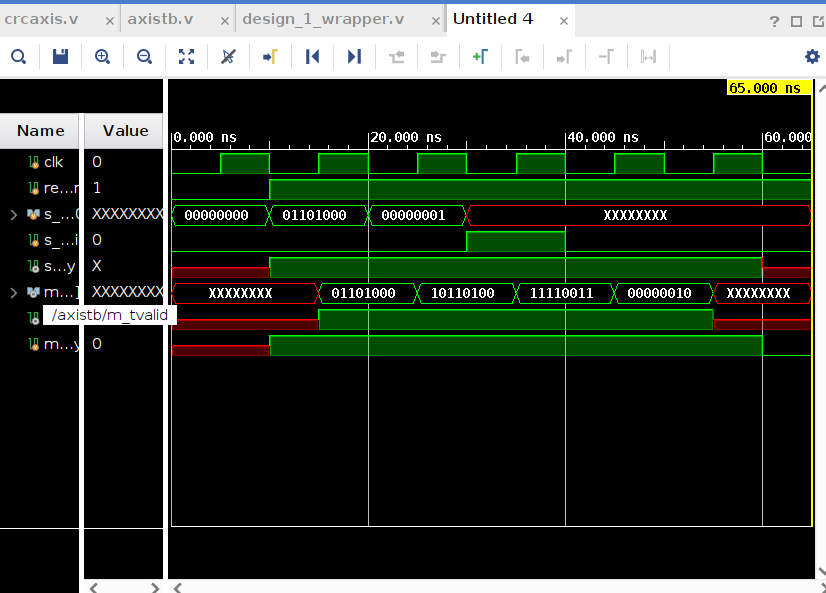
\includegraphics[width=\columnwidth]{figs/p2ipwav.png}
    \caption{Output of IP Testbench}
    \label{fig:my_label}
\end{figure}

\vspace{1cm}
\section{Design Choices}
\vspace{1cm}
\begin{lstlisting}
1. With same design Choices as PART-1, I designed PART-2 by defining all 
I/O buses manually.

\end{lstlisting}
\vspace{15cm}
\maketitle
\hfill \textbf{MATLAB REFERENCE}
\section{Matlab Reference}
\begin{figure}[h]
\centering
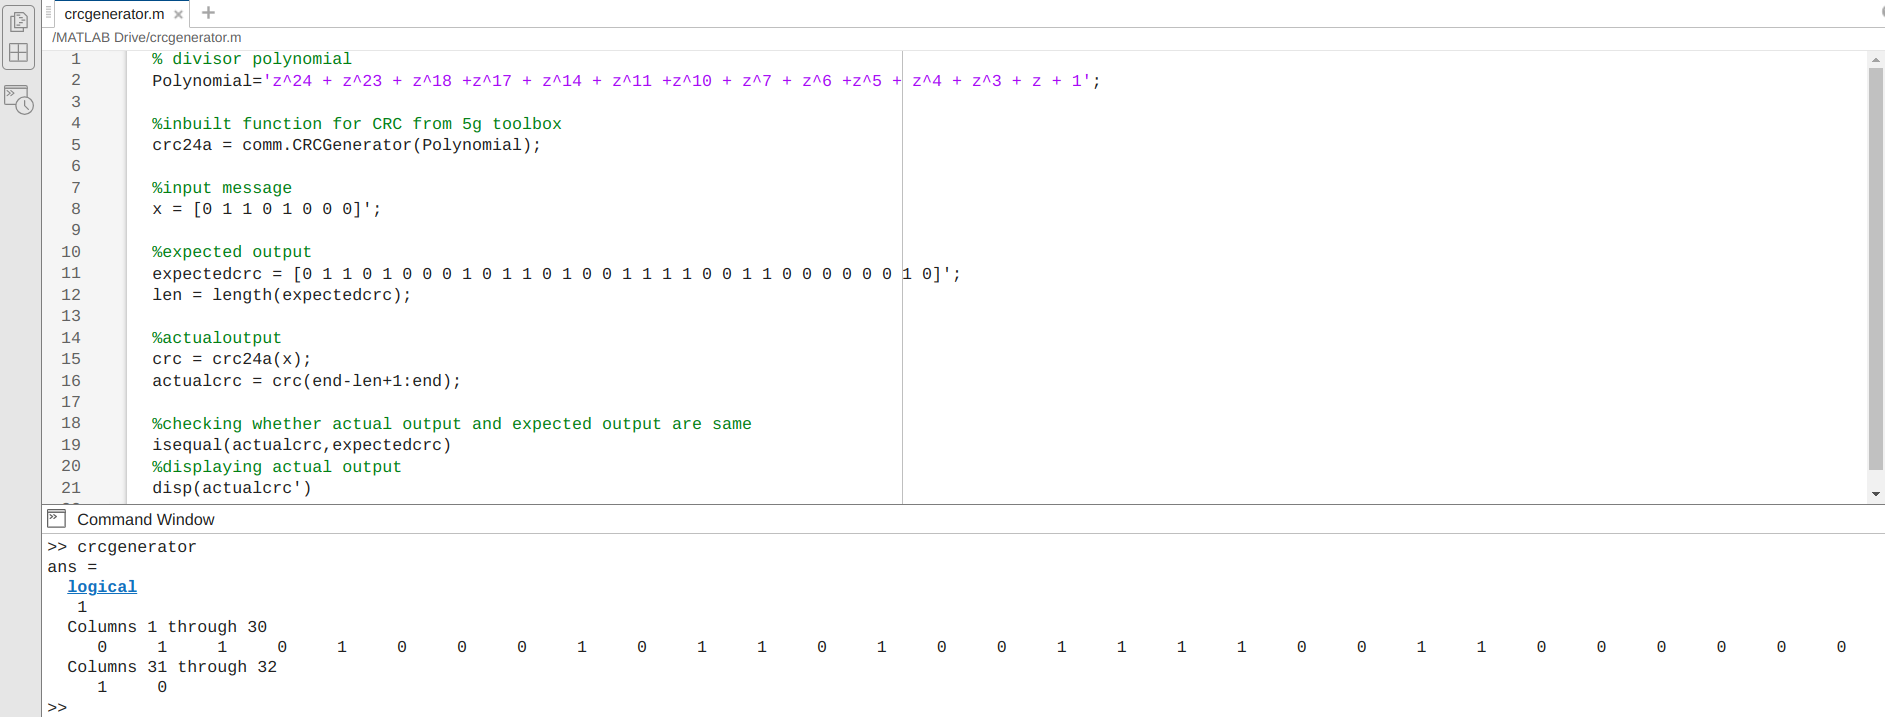
\includegraphics[width=1.3\textwidth]{figs/actual_matlab.png}
    \caption{Matlab Reference}
    \label{fig:my_label}
\end{figure}
\vspace{3cm}
\section{Conclusion}
\begin{lstlisting}
The Output of CRC IP in both PART-1 and Part-2 is matching with Output of 
reference Matlab code and also using this floating Point Converter Online :

\end{lstlisting}
\url{https://www.h-schmidt.net/FloatConverter/IEEE754.html}
\vspace{2cm}
\\
\textbf{GITHUB :} \url{https://github.com/dk-425/Training.git}
\end{document}


